\documentclass[11pt,a4paper]{article}

\newcommand{\tumsoTime}{09:00 น. - 12:00 น.}
\newcommand{\tumsoRound}{1}

\usepackage{../tumso}

\usepackage{xeCJK}
\setCJKmainfont{IPAMincho}
\setCJKsansfont{IPAGothic}
\setCJKmonofont{IPAGothic}

\begin{document}

\begin{problem}{ぼっち・ざ・ろっく}{standard input}{standard output}{1 seconds}{256 megabytes}{100}

Kessoku Band (結束バンド) แปลตรงตัวว่า วงสายรัด เป็นวงร็อกที่ประกอบไปด้วยเด็กมัธยมปลาย และกำลังได้รับความนิยมอย่างมากในช่วงเวลานี้

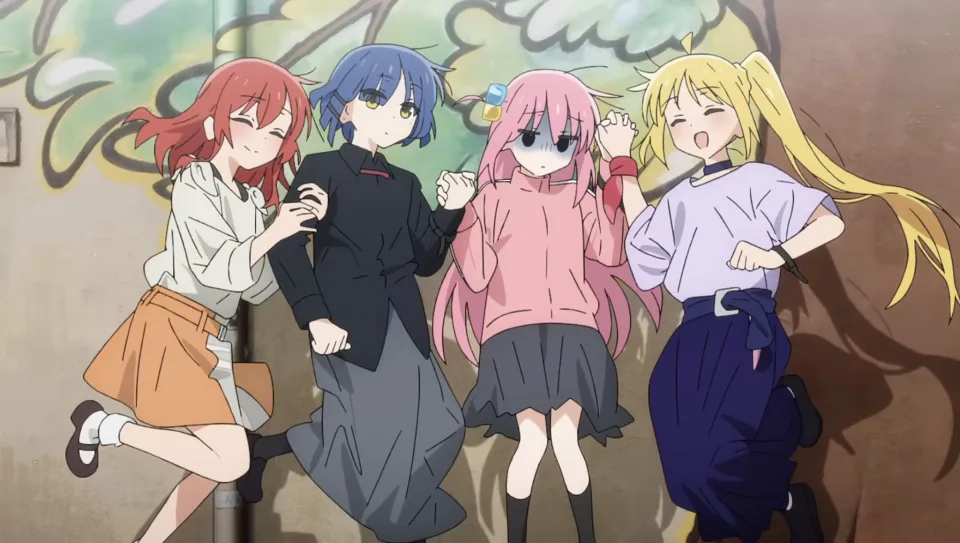
\includegraphics[width=\textwidth]{04-bocchitherock/kessokuband.png}

เราขอแนะนำตัวสมาชิกแต่ละคน เริ่มจากซ้ายไปขวา

喜多郁代 (きた いくよ / Kita Ikuyo) เป็นกีตาร์ร้องนำของวง มีออร่าคิตะคิต้าน ฟุวะ ฟุวะ ปิ้ว ปิ้ว

山田リョウ (やまだ りょう / Yamada Ryou) เป็นมือเบสของวง มักจะช็อตตังแล้วชอบยืมตังชาวบ้าน และกินหญ้าเป็นอาหารเมื่อเงินหมด

後藤ひとり (ごとう ひとり / Gotou Hitori) เป็นมือกีตาร์ของวง เล่นกีตาร์เก่งมาก ๆ ระดับเดียวกับอาจารย์แดง

伊地知虹夏 (いじち にじか / Ijichi Nijika) เป็นมือกลองของวง ร่าเริง ยิ้มแย้มแจ่มใส

เนื่องจากวงนี้ได้รับความนิยมเป็นจำนวนมาก แน่นอนว่าก็มีแฟนคลับ และต่อจากนี้ เราจะมาทำความรู้จักกับแฟนคลับของวงนี้กัน

แฟนคลับท่านแรก ท่านธนพนธ์ ไม่เสื่อมสุข หรือที่รู้จักกันในนาม ToroTN (โตโร่ ทีเอ็น) เป็นบุคคลที่เทพมาก ๆ เคยได้รับรางวัลตั้งใจไม่เสื่อมคลายในการแข่งขันระดับชาติ

แฟนคลับท่านที่สอง ท่านโมกข์ วรรธนะโสภณ หรือที่รู้จักกันในนาม M-W (เอ็ม ดับบิว) เป็นบุคคลที่เทพเช่นกัน เป็นถึงผู้แทนประเทศ ไปแข่งขันระดับนานาชาติที่อินโดนีเซีย ตอนนี้โมกข์กำลังศึกษาอยู่ที่มหาวิทยาลัยแห่งหนึ่งในโตเกียว (東京)

\pagebreak

เมื่อไม่นานมานี้ วง Kessoku ได้ทำการออกซีดีอัลบั้มของวง Kessoku Band 1st Album

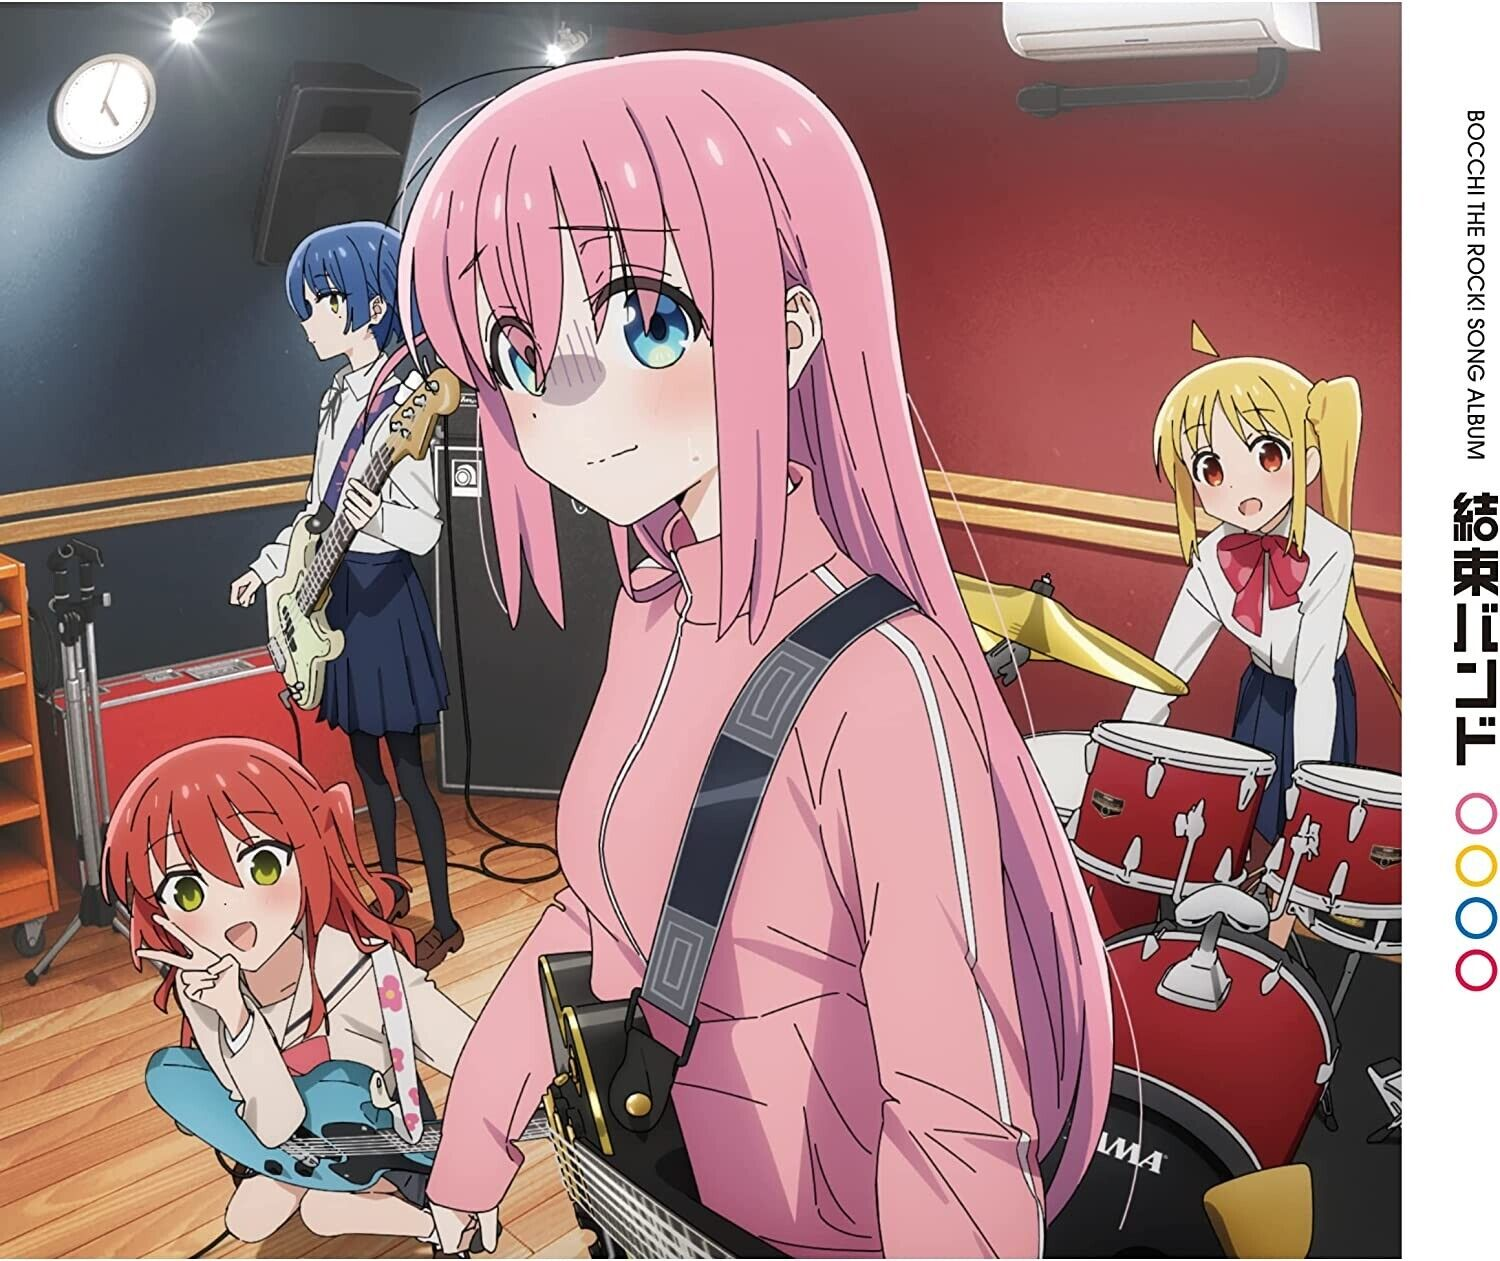
\includegraphics[width=10cm]{04-bocchitherock/kessoku-album.jpg}

แน่นอนว่าแฟนคลับทั้งสองคนนี้ ก็อยากได้สินค้านี้เป็นอย่างมาก ในขณะที่ท่าน M-W ซึ่งเรียนอยู่ที่ญี่ปุ่น สามารถเดินไปในห้างแล้วซื้อแผ่นซีดีได้เลย แต่ท่าน ToroTN ไม่สามารถทำอย่างนั้นได้ เพราะเขาไม่ได้อยู่ญี่ปุ่น

วิธีการที่ดีที่สุดคือการที่ท่าน ToroTN บินไปญี่ปุ่นแล้วพบเจอกับท่าน M-W

ในประเทศญี่ปุ่นจะมีเมืองทั้งหมด $N$ เมือง แต่ละเมืองจะมีเลขกำกับ $0$ ถึง $N-1$ โดยเมืองที่ท่าน M-W อยู่ คือ  東京 (โตเกียว) ซึ่งมีเลขกำกับ $0$ แต่ละเมืองอาจมีถนนเชื่อมกัน โดยจะมีถนนทั้งหมด $M$ เส้น เชื่อมทุกเมืองเข้าด้วยกัน แต่ละเส้นก็มีค่าใช้จ่ายในการเดินทางที่แตกต่างกัน

ในประเทศญี่ปุ่น จะมีสนามบินทั้งหมด $K$ สนามบิน แต่ละเมืองอาจมีหรือไม่มีสนามบินก็ได้ ในการที่จะบินจากกรุงเทพไปยังสนามบินต่าง ๆ ก็มีค่าที่ใช้จ่ายที่แตกต่างกัน ตามเส้นทางการบิน

\YourWork

จงหาค่าใช้จ่ายที่น้อยที่สุดที่ท่าน ToroTN ต้องใช้เพื่อเดินทางไปหาท่าน M-W ที่โตเกียว แล้วก็เดินไปซื้อซีดีอัลบั้มด้วยกันที่อากิฮาบาระ

\pagebreak

\InputFile

บรรทัดแรก จำนวนเต็ม $N$ $(3 \leq N \leq 100\,000)$

บรรทัดที่ $2$ จำนวนเต็ม $M$ $(N - 1 \leq M \leq 200\,000)$

บรรทัดที่ $3$ ถึง $M+2$ จำนวนเต็ม $u_i, v_i, w_i$ แทนว่าถนนเส้นที่ $i$ เชื่อมเมือง $u_i$ และ $v_i$ มีค่าใช้จ่ายในการเดินทาง $w_i$ $(0 \leq w_i \leq 10^6)$

บรรทัดที่ $M+3$ จำนวนเต็ม $K$ แทนจำนวนสนามบิน $(K \leq N)$

บรรทัดที่ $M+4$ ถึง $M+K+3$ จำนวนเต็ม $k, c$ แทนว่ามีเส้นทางการบินจากกรุงเทพไปยังสนามบินที่เมือง $k$ มีค่าใช้จ่าย $c$ $(0 \leq c \leq 10^8)$

\OutputFile

จำนวนเต็มจำนวนเดียว ระบุค่าใช้จ่ายที่น้อยที่สุดที่ใช้ในการเดินทาง เพื่อให้ท่าน ToroTN ไปเจอท่าน M-W ที่โตเกียว

\Scoring
ชุดทดสอบจะถูกแบ่งเป็น 7 ชุด จะได้คะแนนในแต่ละชุดก็ต่อเมื่อโปรแกรมให้ผลลัพธ์ถูกต้องในชุดทดสอบย่อยทั้งหมด

\begin{description}

\item[ชุดที่ 1 (7 คะแนน)] เส้นทางการบินที่ถูกที่สุด บินไปโตเกียว
\item[ชุดที่ 2 (7 คะแนน)] ถนนทุกเส้นไม่มีค่าใช้จ่ายในการเดินทาง
\item[ชุดที่ 3 (31 คะแนน)] $N \leq 5, M \leq 8, K \le 3$
\item[ชุดที่ 4 (19 คะแนน)] $K = 1$
\item[ชุดที่ 5 (22 คะแนน)] $N \le 1\,000, M \leq 5\,000$
\item[ชุดที่ 6 (11 คะแนน)] $N \le 10\,000, M \leq 50\,000$
\item[ชุดที่ 7 (3 คะแนน)] ไม่มีเงื่อนไขเพิ่มเติม

\end{description}

\Examples

\begin{example}
\exmp{4
4
1 0 80
1 2 40
2 0 20
0 3 90
3
1 120
0 200
3 100
}{180
}%
\end{example}

\section*{อธิบายตัวอย่าง}

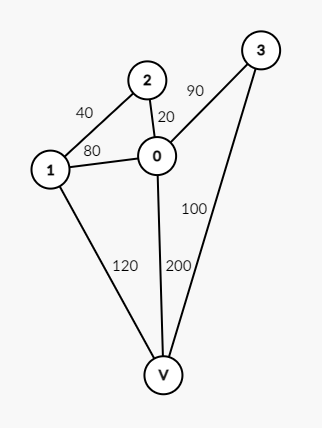
\includegraphics[width=7cm]{04-bocchitherock/bocchitherock-exgraph.png}

นี่คือแผนที่ที่แสดงตัวอย่างที่ให้มา โดย $V$ แทนกรุงเทพ

วิธีการที่ใช้ค่าใช้จ่ายน้อยที่สุดคือการที่ท่าน ToroTN บินมาลงที่เมือง $1$ และเดินทางต่อไปยังเมือง $2$ และไปถึงโตเกียวในที่สุด

\end{problem}

\end{document}
